\chapter{直流电路：基尔霍夫定律与定理}\label{ch:b1:dc-circuits}

寒冷的早晨拧动钥匙：起动机发出呻吟，仪表盘灯
暗了一秒，汽车咳嗽几声便发动起来。那块方才还稳定输出
\qty{12.6}{V} 的电池此刻已降至 11 伏，而
起动机正吸取 150 \omterm{def:b1:dc-circuits:current}{安培}的电流——前大灯
与之并联，也为此付出代价。这一秒内的一切都受
两条守恒定律和若干关于\omterm{def:b1:dc-circuits:linear}{线性电路}的定理所支配，
本章将陈述、证明并应用其中的基尔霍夫定律、
电源与\omterm{def:b1:dc-circuits:resistor}{电阻器}的模型、\omterm{prop:b1:dc-circuits:dividers}{分压器}、戴维南定理和诺顿定理，以及
求\omterm{met:b1:dc-circuits:loadline}{工作点}的图解方法。

\section{电流、电压与准稳态}

\begin{definition}[电流]\label{def:b1:dc-circuits:current}
\index{电流}\index{安培}
通过曲面（导线的横截面）的\emph{电流}，
是单位时间内穿过该面的电荷量，在选定的
正向下取正值：
\[
i = \frac{\dd q}{\dd t} \qquad (\text{安培：} \qty{1}{A} = \qty{1}{C/s}).
\]
改变正向会使 $i$ 变号。在金属中，
载流子是电子，它们的漂移方向与习惯电流方向\emph{相反}，
漂移速率只有每秒零点几毫米。
\end{definition}

\begin{definition}[电势与电压]\label{def:b1:dc-circuits:voltage}
\index{电势}\index{电压}\index{地}
电路中每一点都有一个\emph{电势}$V$（单位为伏特），
其值相差一个常数，该常数由选定的\emph{地}（$V = 0$）确定。
$A$、$B$ 两点之间的\emph{电压}是电势差
$u_{AB} = V_A - V_B$，用由 $B$ 指向 $A$ 的箭头表示。电荷
$q$ 由 $A$ 移到 $B$ 时失去的能量为 $q\,u_{AB}$（这与
\cref{ch:b1:potential-capacitors}中的静电势相联系）。
\end{definition}

\begin{definition}[准稳态（ARQS）]\label{def:b1:dc-circuits:arqs}
\index{准稳态}\index{ARQS}
尺度为 $\ell$、工作频率为 $f$ 的电路处于
\emph{准稳态}，即电\omterm{def:b1:wave-propagation:signal}{信号}沿电路传播所需的时间 $\ell/c$
与周期 $1/f$ 相比可以忽略：
$\ell \ll c/f$。此时，无分支导线上各点的电流在每一瞬间相同，
下述定律在每一瞬间
对随时间变化的电流与\omterm{def:b1:dc-circuits:voltage}{电压}（小写的 $i$、$u$）成立，
其形式与对稳恒量（$I$、$U$）的情形完全相同。
\end{definition}

\begin{example}[准稳态有多准]\label{ex:b1:dc-circuits:arqs}
频率为 \qty{50}{Hz} 时，$c/f = \qty{6000}{km}$：房屋处于
\omterm{def:b1:dc-circuits:arqs}{准稳态}；频率为 \qty{1}{MHz} 时为 \qty{300}{m}，收音机仍然如此；频率为 \qty{2}{GHz} 时，
\qty{15}{cm}：手机电路板则不然，其走线必须
当作传输线处理，这是本科二年级分册的内容。
\end{example}

\begin{theorem}[基尔霍夫定律]\label{thm:b1:dc-circuits:kirchhoff}
\index{基尔霍夫定律}\index{节点定律}\index{回路定律}
\omterm{def:b1:dc-circuits:arqs}{准稳态}下有：
\begin{enumerate}
  \item \emph{节点定律}：在多根导线汇合的节点处，流入的电流之和
        等于流出的电流之和，
        $\sum_{\text{入}} i_k = \sum_{\text{出}} i_k$。
  \item \emph{回路定律}：沿任一闭合回路，各\omterm{def:b1:dc-circuits:voltage}{电压}的代数和
        在按所选绕行方向取符号后为零：
        $\sum_{\text{回路}} \pm u_k = 0$。
\end{enumerate}
\end{theorem}

\begin{proof}
电荷守恒，且在\omterm{def:b1:dc-circuits:arqs}{准稳态}下电荷不会在节点处堆积：
每秒流入的电荷恰等于每秒流出的电荷。回路定律
即\omterm{def:b1:dc-circuits:voltage}{电势}是位置的函数：绕回路一周
回到出发点时，\omterm{def:b1:dc-circuits:voltage}{电势}降落之和
为 $V_A - V_A = 0$。
\end{proof}

\begin{notation}[约定与功率]\label{not:b1:dc-circuits:conventions}
\index{受电器约定}\index{发电器约定}\index{电功率}
对于二端元件（\emph{偶极子}），\emph{\omterm{thm:b1:dc-circuits:kirchhoff}{受电器
约定}}中\omterm{def:b1:dc-circuits:voltage}{电压}箭头与电流箭头方向相反；
\emph{\omterm{thm:b1:dc-circuits:kirchhoff}{发电器约定}}中两者方向相同。在\omterm{thm:b1:dc-circuits:kirchhoff}{受电器约定}下，偶极子
\emph{接收}的功率为
%
\[
p = u\,i \qquad (\text{瓦特}),
\]
对于发热的\omterm{def:b1:dc-circuits:resistor}{电阻器}为正，对于
向外供电的电池为负。在\omterm{thm:b1:dc-circuits:kirchhoff}{发电器约定}下，$p = ui$ 是偶极子
\emph{输出}的功率。
\end{notation}

\begin{omfigure}
\begin{tikzpicture}[font=\small]
  \draw (0,0) to[generic, l=偶极子, v=$u$, i=$i$] (3,0);
  \node[below] at (1.5,-1.0) {受电器约定：$p_{\text{接收}} = ui$};
  \begin{scope}[xshift=6cm]
  \draw (0,0) to[generic, l=偶极子, v<=$u$, i=$i$] (3,0);
  \node[below] at (1.5,-1.0) {发电器约定：$p_{\text{输出}} = ui$};
  \end{scope}
\end{tikzpicture}

{\small 偶极子的两种符号约定：箭头相反
（受电器）或相同（发电器）。二者的物理内容相同，只是
对 $ui$ 符号的解读方式不同。}
\end{omfigure}

\section{偶极子及其模型}

\begin{definition}[伏安特性；电阻器；欧姆定律]\label{def:b1:dc-circuits:resistor}
\index{伏安特性（偶极子的）}\index{电阻器}\index{欧姆定律}\index{焦耳效应}
偶极子的\emph{伏安特性}是其所施加的曲线 $i(u)$
（或 $u(i)$）。\emph{电阻器}的伏安特性是过原点的直线，
即\emph{欧姆定律}
\[
u = R\,i \qquad (\text{受电器约定}),
\]
$R$ 为其\emph{电阻}（单位为欧姆，$\qty{1}{\ohm} = \qty{1}{V/A}$），
$G = 1/R$ 为其\emph{电导}（单位为西门子）。它接收的功率为 $p = Ri^2 =
u^2/R \geq 0$，以热量形式耗散（\emph{焦耳效应}）。一段
长为 $\ell$、横截面积为 $S$、电阻率为 $\rho$ 的导线，
其电阻为 $R = \rho\ell/S$。
\end{definition}

\begin{definition}[理想电源与实际电源]\label{def:b1:dc-circuits:sources}
\index{电压源}\index{电流源}\index{电动势}\index{内阻}\index{戴维南模型}\index{诺顿模型}
\emph{理想\omterm{def:b1:dc-circuits:voltage}{电压}源}使 $u = E$，无论电流为何值；
$E$ 为其\emph{电动势}。\emph{理想电流
源}使 $i = I_N$，与\omterm{def:b1:dc-circuits:voltage}{电压}无关。\emph{实际电源}
（电池、发电机、电源）在发电机约定下，
可由下式建模：
\[
u = E - r\,i \quad (\text{戴维南模型：理想电动势 } E \text{ 串联于 } r)
\]
或等价地，由 $i = I_N - u/r$ 描述（诺顿模型：理想电流
源 $I_N = E/r$ 与 $r$ 并联）；$r$ 为\emph{内
阻}。$E$ 为开路\omterm{def:b1:dc-circuits:voltage}{电压}，$I_N = E/r$ 为
短路电流。
\end{definition}

\begin{proposition}[实际电源的功率平衡]\label{prop:b1:dc-circuits:sourcepower}
\index{最大功率传输}
实际电源 $(E, r)$ 向\omterm{def:b1:dc-circuits:resistor}{电阻器} $R$ 供电时，电流 $i = E/(R + r)$，
其功率为
\[
P_R = \frac{E^2 R}{(R + r)^2},
\]
功率最大，为 $E^2/4r$，此时 $R = r$（\emph{阻抗匹配}），
效率 $P_R/(Ei) = R/(R + r)$，最大时仅为 $50\%$。
\end{proposition}

\begin{proof}
回路定律：$E = ri + Ri$。$P_R = Ri^2$；对 $R/(R + r)^2$ 求导：
$\big[(R + r)^2 - 2R(R + r)\big]/(R + r)^4 = (r - R)/(R + r)^3$，
当 $R = r$ 时为零，之前为正，之后为负。电源提供
$Ei = (R + r)i^2$，其中 $ri^2$ 使电源自身发热。
\end{proof}

\begin{omfigure}
\begin{tikzpicture}
\begin{axis}[omaxis, width=7.6cm, height=5.2cm, xlabel={$i$}, ylabel={$u$},
    xmin=0, xmax=1.3, ymin=0, ymax=1.3, xtick={1}, xticklabels={$I_N = E/r$},
    ytick={1}, yticklabels={$E$}]
  \addplot[omThm, thick, domain=0:1, samples=2] {1 - x};
  \addplot[omDef, thick, domain=0:0.9, samples=2] {0.6*x};
  \fill[omExo] (axis cs:0.625,0.375) circle (1.6pt);
  \node[omExo, font=\footnotesize] (op) at (axis cs:0.98,0.92) {工作点};
  \draw[-Stealth, omExo] (op.south west) -- (axis cs:0.645,0.395);
  \node[omThm, font=\footnotesize, anchor=south west] at (axis cs:0.03,1.02) {电源 $u = E - ri$};
  \node[omDef, font=\footnotesize, right] at (axis cs:0.9,0.54) {负载 $u = Ri$};
\end{axis}
\end{tikzpicture}\qquad
\begin{tikzpicture}
\begin{axis}[omaxis, width=7.0cm, height=5cm, xlabel={$R/r$}, ylabel={$P_R$},
    xmin=0, xmax=6, ymin=0, ymax=0.3, xtick={1,3,5}, ytick={0.25}, yticklabels={$\frac{E^2}{4r}$}]
  \addplot[omProp, thick, domain=0:6, samples=120] {x/((x+1)^2)};
  \draw[dashed, omExo] (axis cs:1,0) -- (axis cs:1,0.25) -- (axis cs:0,0.25);
\end{axis}
\end{tikzpicture}

{\small 左图：实际电源（$u = E - ri$）的伏安特性与
电阻性负载（$u = Ri$）的伏安特性相交于\omterm{met:b1:dc-circuits:loadline}{工作点}。右图：负载
获得的功率在 $R = r$ 处达到峰值，此时
电源有一半功率消耗在自身\omterm{def:b1:dc-circuits:sources}{内阻}上。}
\end{omfigure}

\begin{example}[负载下的汽车电池]\label{ex:b1:dc-circuits:battery}
开路\omterm{def:b1:dc-circuits:voltage}{电压}为 \qty{12.6}{V}；起动电动机抽取
\qty{120}{A} 电流时\omterm{def:b1:dc-circuits:voltage}{电压}为 \qty{11.4}{V}：$r = 1.2/120 = \qty{10}{m\ohm}$，$I_N = \qty{1260}{A}$
（因此扳手不慎掉落时的危险堪比焊接）。匹配负载
$R = \qty{10}{m\ohm}$ 时将取用功率 $E^2/4r = \qty{4}{kW}$，持续
几秒钟——大致相当于起动电动机所需的功率。
\end{example}

\begin{remark}[其他二端元件]\label{rem:b1:dc-circuits:others}
\index{二极管}
\emph{二极管}只沿一个方向导通：其理想模型在 $u < U_0$ 时为
断路；导通时\omterm{def:b1:dc-circuits:voltage}{电压}固定为 $u = U_0$（
硅管约 \qty{0.7}{V}，发光二极管约 \qty{2}{} 至 \qty{3}{V}）。
白炽灯是一种\omterm{def:b1:dc-circuits:resistor}{电阻器}，其 $R$ 随
温度升高而增大，因而也随 $i$ 变化，具有曲线形伏安特性。稳态时
电容器相当于断开的电路（$i = C\,\dd u/\dd t = 0$），而
电感器相当于短路（$u = L\,\dd i/\dd t = 0$）；它们在
暂态中的作用见\cref{ch:b1:transient-regimes}。
\end{remark}

\section{电阻的连接与分压、分流}

\begin{proposition}[串联与并联电阻器]\label{prop:b1:dc-circuits:seriesparallel}
\index{串联电阻}\index{并联电阻}
\omterm{prop:b1:dc-circuits:seriesparallel}{串联电阻}器（电流相同）的电阻相加：$R = R_1 + R_2 + \cdots$。
\omterm{prop:b1:dc-circuits:seriesparallel}{并联电阻}器（\omterm{def:b1:dc-circuits:voltage}{电压}相同）的电导相加：
$1/R = 1/R_1 + 1/R_2 + \cdots$；对两个电阻，$R = R_1R_2/(R_1 + R_2)$，
记作 $R_1 \parallel R_2$。
\end{proposition}

\begin{proof}
串联：$u = u_1 + u_2 = (R_1 + R_2)i$（由回路定律）。并联：$i = i_1 +
i_2 = u/R_1 + u/R_2$（由节点定律）。
\end{proof}

\begin{proposition}[分压器与分流器]\label{prop:b1:dc-circuits:dividers}
\index{分压器}\index{分流器}
两个串联在\omterm{def:b1:dc-circuits:voltage}{电压} $u$ 两端的\omterm{def:b1:dc-circuits:resistor}{电阻器}按
其阻值之比分配该\omterm{def:b1:dc-circuits:voltage}{电压}：
\[
u_2 = \frac{R_2}{R_1 + R_2}\,u .
\]
两个并联、由电流 $i$ 供电的\omterm{def:b1:dc-circuits:resistor}{电阻器}，按
电阻的反比分配该电流：
\[
i_2 = \frac{R_1}{R_1 + R_2}\,i = \frac{G_2}{G_1 + G_2}\,i .
\]
\end{proposition}

\begin{proof}
串联时：$i = u/(R_1 + R_2)$，且 $u_2 = R_2 i$。并联时：$u = (R_1
\parallel R_2)\,i$，且 $i_2 = u/R_2$。
\end{proof}

\begin{omfigure}
\begin{tikzpicture}[font=\small]
  \draw (0,3.2) to[R=$R_1$] (0,1.6) to[R=$R_2$, v=$u_2$] (0,0);
  \draw[-Stealth, thick] (-1.3,0.1) -- (-1.3,3.1) node[midway, left] {$u$};
  \fill (0,3.2) circle (1.2pt); \fill (0,0) circle (1.2pt);
  \begin{scope}[xshift=5.5cm]
  \draw (0,3.2) to[short, i=$i$] (1.4,3.2) to[R=$R_1$] (1.4,0) -- (0,0);
  \draw (1.4,3.2) -- (3.0,3.2) to[short, i=$i_2$] (3.0,2.4) to[R=$R_2$] (3.0,0) -- (1.4,0);
  \fill (0,3.2) circle (1.2pt); \fill (0,0) circle (1.2pt);
  \end{scope}
\end{tikzpicture}

{\small \omterm{prop:b1:dc-circuits:dividers}{分压器}（左）：$u_2 = R_2 u/(R_1 + R_2)$。\omterm{prop:b1:dc-circuits:dividers}{分流器}
（右）：$i_2 = R_1 i/(R_1 + R_2)$——电流更倾向于流过
较小的电阻。}
\end{omfigure}

\begin{remark}[分压器的负载]\label{rem:b1:dc-circuits:loading}
分压公式只在中点不向外分出电流时成立。
将负载 $R_L$ 接在 $R_2$ 两端时，$R_2$ 被等效为 $R_2
\parallel R_L$，$u_2$ 随之降低——这就是“负载效应”，也是
\omterm{def:b1:dc-circuits:voltage}{电压}表的电阻必须远大于、而电位器的电阻必须远小于
其所连接的电路的原因
（见\cref{exo:b1:dc-circuits:4}）。
\end{remark}

\begin{method}[化简网络]\label{met:b1:dc-circuits:reduce}
求含若干电阻和一个电源的网络中某一电流或\omterm{def:b1:dc-circuits:voltage}{电压}
时：
\begin{enumerate}
  \item 从远离电源处开始，将串联组与并联组替换为等效电阻，
        直到只剩一个电阻与
        电源相连；
  \item 计算电源输出的电流；
  \item 逐级回推，用\omterm{prop:b1:dc-circuits:dividers}{分流器}分配电流、
        用\omterm{prop:b1:dc-circuits:dividers}{分压器}分配\omterm{def:b1:dc-circuits:voltage}{电压}，直到所求支路。
\end{enumerate}
若有多个电源，或所求支路的相邻元件会改变，则使用
下一节的定理。
\end{method}

\section{线性电路定理}

\begin{definition}[线性二端元件、线性电路]\label{def:b1:dc-circuits:linear}
\index{线性二端元件}
若二端元件的伏安特性为一条直线，则称其为\emph{线性}元件
（\omterm{def:b1:dc-circuits:resistor}{电阻器}、理想电源和实际电源）；仅由线性二端元件构成的电路
称为\emph{线性电路}。其未知量满足一组
线性方程（基尔霍夫定律加上各元件的伏安特性），其
解唯一。
\end{definition}

\begin{theorem}[戴维南定理与诺顿定理]\label{thm:b1:dc-circuits:thevenin}
\index{戴维南定理}\index{诺顿定理}
从其两个接线端 $A$ 和 $B$ 看去，任一\omterm{def:b1:dc-circuits:linear}{线性电路}都
等效于一个实际电源：\omterm{def:b1:dc-circuits:sources}{电动势} $E_{\mathrm{Th}}$ 与
电阻 $R_{\mathrm{Th}}$ 串联（戴维南等效），或\omterm{def:b1:dc-circuits:sources}{电流源} $I_N =
E_{\mathrm{Th}}/R_{\mathrm{Th}}$ 与 $R_{\mathrm{Th}}$ 并联
（诺顿等效），其中
\begin{itemize}
  \item $E_{\mathrm{Th}}$ 为开路\omterm{def:b1:dc-circuits:voltage}{电压} $u_{AB}$；
  \item $I_N$ 为从 $A$ 到 $B$ 的短路电流；
  \item $R_{\mathrm{Th}}$ 为将所有独立电源关闭（理想\omterm{def:b1:dc-circuits:sources}{电压源}
        以导线代替，理想\omterm{def:b1:dc-circuits:sources}{电流源}
        以断路代替）后，从 $A$ 和 $B$ 之间
        看去的电阻。
\end{itemize}
\end{theorem}

\begin{proof}[部分证明]
由线性性，\omterm{def:b1:dc-circuits:voltage}{电压} $u_{AB}$ 与从接线端引出的电流
$i$ 之间的关系是仿射的：$u_{AB} = a - b\,i$。令
$i = 0$ 得 $a = E_{\mathrm{Th}}$；令 $u_{AB} = 0$ 得
$b = E_{\mathrm{Th}}/I_N$。$b$ 等于关闭电源后所见的电阻，
这由叠加定理（见下文）得出：$u_{AB}$ 中
仅由外部电流产生的部分，正是阻值为
$R_{\mathrm{Th}}$ 的无源网络所产生的。任一线性系统都具有
仿射的输入—输出关系，这是线性方程组的代数结论。
\end{proof}

\begin{theorem}[叠加定理]\label{thm:b1:dc-circuits:superposition}
\index{叠加定理}
在含有若干独立电源的\omterm{def:b1:dc-circuits:linear}{线性电路}中，任一电流或
\omterm{def:b1:dc-circuits:voltage}{电压}都等于各电源单独作用时所取值之和，
此时其余电源均关闭。
\end{theorem}

\begin{proof}
方程对未知量是线性的，电源构成
右端项；解是该右端项的线性函数，
因此等于对各电源分别求解所得之和。
\end{proof}

\begin{proposition}[米尔曼定理]\label{prop:b1:dc-circuits:millman}
\index{米尔曼定理}
节点 $N$ 与\omterm{def:b1:dc-circuits:voltage}{电势}为 $V_1, \dots, V_n$ 的各点分别
通过电阻 $R_1, \dots, R_n$ 相连（且不与其他任何元件相连），其\omterm{def:b1:dc-circuits:voltage}{电势}为
\[
V_N = \frac{\sum_k V_k/R_k}{\sum_k 1/R_k} = \frac{\sum_k G_k V_k}{\sum_k G_k},
\]
即其相邻各点\omterm{def:b1:dc-circuits:voltage}{电势}以电导为权的加权平均。
\end{proposition}

\begin{proof}
在 $N$ 处应用节点定律：$\sum_k (V_k - V_N)/R_k = 0$；解出 $V_N$ 即可。
\end{proof}

\begin{omfigure}
\begin{tikzpicture}[font=\small]
  % network: E1=10V, R1=1k ; E2=5V, R2=2k ; common load R3=2k
  \draw (0,0) to[battery1, l=$E_1$, invert] (0,2) to[R=$R_1$] (2.5,2) -- (2.5,2) to[R=$R_3$, v=$u$] (2.5,0) -- (0,0);
  \draw (2.5,2) to[R=$R_2$] (5,2) to[battery1, l_=$E_2$] (5,0) -- (2.5,0);
  \node at (2.5,2.45) {$N$};
  \node at (6.4,1) {$\Longleftrightarrow$};
  \begin{scope}[xshift=8.8cm]
  \draw (0,0) to[battery1, l=$E_{\mathrm{Th}}$, invert] (0,2) to[R=$R_{\mathrm{Th}}$] (2.2,2) to[R=$R_3$, v=$u$] (2.2,0) -- (0,0);
  \end{scope}
\end{tikzpicture}

{\small 两个电源向公共负载 $R_3$ 供电。从 $R_3$ 两端看去，
电路其余部分等效为戴维南电源
（$E_{\mathrm{Th}}$，$R_{\mathrm{Th}}$）；由米尔曼定理可一步求得
节点 $N$ 的\omterm{def:b1:dc-circuits:voltage}{电势}。}
\end{omfigure}

\begin{example}[同一结果的三种求法]\label{ex:b1:dc-circuits:threeways}
图中 $E_1 = \qty{10}{V}$，$R_1 = \qty{1.0}{k\ohm}$，$E_2 =
\qty{5.0}{V}$，$R_2 = \qty{2.0}{k\ohm}$，$R_3 = \qty{2.0}{k\ohm}$。
\emph{米尔曼}：$V_N = (10/1 + 5/2 + 0/2)/(1 + 0.5 + 0.5) = 12.5/2 =
\qty{6.25}{V}$。\emph{叠加}：仅 $E_1$ 作用时，$R_2 \parallel
R_3 = \qty{1}{k\ohm}$，故 $u = 10 \times 1/2 = \qty{5}{V}$；仅 $E_2$ 作用时，
$R_1 \parallel R_3 = \qty{0.667}{k\ohm}$，$u = 5 \times 0.667/2.667
= \qty{1.25}{V}$；合计 \qty{6.25}{V}。\emph{戴维南}：从
$R_3$ 处看去：$E_{\mathrm{Th}}$ 为\omterm{prop:b1:dc-circuits:dividers}{分压器}
$(E_1, R_1, R_2, E_2)$ 的开路\omterm{def:b1:dc-circuits:voltage}{电压}：$E_2 + (E_1 - E_2)R_2/(R_1 + R_2) = 5 + 5 \times
2/3 = \qty{8.33}{V}$；$R_{\mathrm{Th}} = R_1 \parallel R_2 =
\qty{0.667}{k\ohm}$；于是 $u = 8.33 \times 2/2.667 = \qty{6.25}{V}$。
\end{example}

\section{工作点；惠斯通电桥}

\begin{method}[图解法求工作点]\label{met:b1:dc-circuits:loadline}
\index{工作点}\index{负载线}
非\omterm{def:b1:dc-circuits:linear}{线性二端元件}（伏安关系 $i = g(u)$）由戴维南电源
$(E, R)$ 供电时，两个关系同时成立之处即为其工作状态：画出二端元件的
伏安特性曲线与电源的\emph{\omterm{met:b1:dc-circuits:loadline}{负载线}} $u = E - Ri$ 画在同一坐标轴上，
二者的交点即为\emph{\omterm{met:b1:dc-circuits:loadline}{工作点}}。设计
发光二极管的\omterm{prop:b1:dc-circuits:seriesparallel}{串联电阻}、稳压二极管的稳压电路或晶体管的偏置，
正是这一作图过程。
\end{method}

\begin{omfigure}
\begin{tikzpicture}
\begin{axis}[omaxis, width=8cm, height=5.4cm, xlabel={$u$ (\unit{V})}, ylabel={$i$ (\unit{mA})},
    xmin=0, xmax=5.6, ymin=0, ymax=30, xtick={1,2,3,4,5}, ytick={10,20,25}]
  \addplot[omDef, thick, domain=0:1.9, samples=2] {0};
  \addplot[omDef, thick, domain=1.9:2.9, samples=60] {28*(exp(2.8*(x-1.9))-1)/(exp(2.8)-1)};
  \addplot[omThm, thick, domain=0:5, samples=2] {25 - 5*x};
  \fill[omExo] (axis cs:2.0,15) circle (1.6pt);
  \node[omExo, font=\footnotesize] (op) at (axis cs:1.05,11.5) {工作点};
  \draw[-Stealth, omExo] (op.east) -- (axis cs:1.93,14.8);
  \node[omDef, font=\footnotesize, left] at (axis cs:2.55,25) {发光二极管};
  \node[omThm, font=\footnotesize] at (axis cs:3.1,1.4) {负载线};
\end{axis}
\end{tikzpicture}

{\small 发光二极管（开启\omterm{def:b1:dc-circuits:voltage}{电压}约 \qty{2}{V}）由 $E = \qty{5}{V}$ 经
$R = \qty{200}{\ohm}$ 供电：\omterm{met:b1:dc-circuits:loadline}{负载线} $u = E - Ri$ 与
二极管的伏安特性曲线交于 $\qty{2.0}{V}$、\qty{15}{mA} 处。增大 $R$
会使\omterm{met:b1:dc-circuits:loadline}{负载线}向下倾斜，发光二极管变暗。}
\end{omfigure}

\begin{proposition}[惠斯通电桥]\label{prop:b1:dc-circuits:wheatstone}
\index{惠斯通电桥}
四个电阻 $R_1, R_2$（一条支路）与 $R_3, R_4$（另一条支路）接在
电源 $E$ 两端，电桥输出为两中点间的
\omterm{def:b1:dc-circuits:voltage}{电压}：
\[
u = E\left(\frac{R_2}{R_1 + R_2} - \frac{R_4}{R_3 + R_4}\right),
\]
输出为零（此时电桥称为\emph{平衡}的）的充要条件是 $R_1R_4 = R_2R_3$。对于
平衡电桥，若 $R_4$ 变为 $R_4(1 + \epsilon)$，$\epsilon
\ll 1$，且 $R_3 = R_4$，则 $u \approx -E\epsilon/4$。
\end{proposition}

\begin{proof}
两个\omterm{prop:b1:dc-circuits:dividers}{分压器}作差。平衡条件：$R_2(R_3 + R_4) = R_4(R_1 +
R_2)$，即 $R_2R_3 = R_1R_4$。取 $R_3 = R_4 = R$，$R_1 = R_2$，则
$u = E[\tfrac12 - (1 + \epsilon)/(2 + \epsilon)] = E[(2 + \epsilon - 2 -
2\epsilon)/(2(2 + \epsilon))] \approx -E\epsilon/4$.
\end{proof}

\begin{omfigure}
\begin{tikzpicture}[font=\small]
  \draw (0,1.5) to[R=$R_1$] (2,3) to[R=$R_2$] (4,1.5) to[R=$R_4$] (2,0) to[R=$R_3$] (0,1.5);
  \draw (2,3) to[short, *-] (2,3); \draw (2,0) to[short, *-] (2,0);
  \draw (0,1.5) -- (-1,1.5) to[battery1, l=$E$] (-1,-1) -- (4,-1) -- (4,1.5);
  \draw[-Stealth, omThm] (2,0.35) -- (2,2.65) ;
  \node[omThm, right] at (2.05,1.5) {$u$};
\end{tikzpicture}

{\small \omterm{prop:b1:dc-circuits:wheatstone}{惠斯通电桥}：两个分压电路并排放置。电桥平衡时
$R_1R_4 = R_2R_3$，它能把某一电阻的微小变化（应变片、热敏电阻）
转换为接近零的\omterm{def:b1:dc-circuits:voltage}{电压}，
这比放大大\omterm{def:b1:dc-circuits:voltage}{电压}上的微小变化容易得多。}
\end{omfigure}

\section{练习}

\begin{exercise}[$\star$]\label{exo:b1:dc-circuits:1}
手机以 \qty{1.5}{A} 的电流充电一小时：流过的电荷量是多少，
有多少个电子通过？估算下列情形中\omterm{def:b1:dc-circuits:arqs}{准稳态}近似是否成立：
频率为 \qty{50}{Hz} 的家庭线路、长 \qty{10}{cm} 的电路在 \qty{1}{MHz} 时，
以及同一电路在 \qty{1}{GHz} 时。
\end{exercise}

\begin{exercise}[$\star$]\label{exo:b1:dc-circuits:2}
\qty{2000}{W} 的电热器接在 \qty{230}{V} 电源上：求其电流、电阻，以及
在 \qty{3.0}{h} 内消耗的能量（分别以 kWh 和焦耳表示）。其 \qty{5.0}{m} 长的铜导线
横截面积为 \qty{1.5}{mm^2}（$\rho = \qty{1.7e-8}{\ohm.m}$），求
导线上损耗的功率。
\end{exercise}

\begin{exercise}[$\star$]\label{exo:b1:dc-circuits:3}
求 $\qty{10}{\ohm}$、$\qty{20}{\ohm}$ 和 $\qty{30}{\ohm}$ 三个电阻的
串联与并联等效电阻，以及
$(10 \parallel 20) + 30$ 的等效电阻。
\end{exercise}

\begin{exercise}[$\star$]\label{exo:b1:dc-circuits:4}
一个 \qty{12}{V} 电源向串联的 \qty{4.7}{k\ohm} 和 \qty{2.2}{k\ohm} 电阻供电。
求 \qty{2.2}{k\ohm} 电阻两端的\omterm{def:b1:dc-circuits:voltage}{电压}。一个
阻值为 \qty{2.2}{k\ohm} 的器件随后并接在其两端：新的\omterm{def:b1:dc-circuits:voltage}{电压}是多少？
由此说明负载效应。
\end{exercise}

\begin{exercise}[$\star\star$]\label{exo:b1:dc-circuits:5}
一节电池开路时读数为 \qty{12.6}{V}，输出
\qty{120}{A} 电流时读数为 \qty{11.4}{V}。求其\omterm{def:b1:dc-circuits:sources}{内阻}与短路电流，
供给起动机的功率、电池内部损耗的功率，以及
效率。
\end{exercise}

\begin{exercise}[$\star\star$]\label{exo:b1:dc-circuits:6}
从 \qty{2.2}{k\ohm} 电阻两端看进去，求
\cref{exo:b1:dc-circuits:4} 中\omterm{prop:b1:dc-circuits:dividers}{分压器}的戴维南等效电路
（$E = \qty{12}{V}$，$R_1 = \qty{4.7}{k\ohm}$，$R_2 = \qty{2.2}{k\ohm}$）。
利用它求出该题中的负载\omterm{def:b1:dc-circuits:voltage}{电压}。
\end{exercise}

\begin{exercise}[$\star\star$]\label{exo:b1:dc-circuits:7}
两节电池 $E_1 = \qty{10}{V}$（$r_1 = \qty{1.0}{\ohm}$）与
$E_2 = \qty{5.0}{V}$（$r_2 = \qty{2.0}{\ohm}$）同极性并联
后跨接在 \qty{2.0}{\ohm} 负载两端。求
负载\omterm{def:b1:dc-circuits:voltage}{电压}，先用叠加原理、再用米尔曼定理，以及
每节电池中的电流。较弱的电池是在充电还是放电？
\end{exercise}

\begin{exercise}[$\star\star$]\label{exo:b1:dc-circuits:8}
电源 $E = \qty{9.0}{V}$，$r = \qty{3.0}{\ohm}$。求其
向阻值为 $\qty{1.0}{\ohm}$、$\qty{3.0}{\ohm}$、$\qty{12}{\ohm}$ 的负载输出的功率，
以及各情形下的效率。对于电池供电的器件，
工程师会选择哪一个负载？为什么不选匹配负载？
\end{exercise}

\begin{exercise}[$\star\star$]\label{exo:b1:dc-circuits:9}
一只发光二极管在 \qty{2.0}{V} 时导通，需要由
\qty{5.0}{V} 电源供电，通过 \qty{15}{mA} 的电流。选择\omterm{prop:b1:dc-circuits:seriesparallel}{串联电阻}，
求电阻与二极管各自消耗的功率，并画出\omterm{met:b1:dc-circuits:loadline}{负载线}的作图过程。
若电源为 \qty{3.3}{V}，会出现什么情况？
\end{exercise}

\begin{exercise}[$\star\star\star$]\label{exo:b1:dc-circuits:10}
应变片 $R_4 = R(1 + \epsilon)$，$R = \qty{1.0}{k\ohm}$，接于一个
\omterm{prop:b1:dc-circuits:wheatstone}{惠斯通电桥}中，该桥另有三个固定的 \qty{1.0}{k\ohm} 电阻，
并接在 \qty{5.0}{V} 电源两端。推导关于 $\epsilon$ 的一阶近似输出\omterm{def:b1:dc-circuits:voltage}{电压}，
并计算 $\epsilon = \num{1.0e-3}$ 时的值。为什么电桥
比在简单\omterm{prop:b1:dc-circuits:dividers}{分压器}中测量应变片\omterm{def:b1:dc-circuits:voltage}{电压}更为可取？
\end{exercise}

\begin{exercise}[$\star\star\star$]\label{exo:b1:dc-circuits:11}
十二个相同的电阻 $R$ 构成一个正方体的棱。利用对称性（判断当电流 $I$ 在一个顶点流入、
在其对角顶点流出时，哪些节点具有相同的\omterm{def:b1:dc-circuits:voltage}{电势}），
证明相对顶点之间的
电阻为 $5R/6$。
\end{exercise}

\begin{exercise}[$\star\star\star$]\label{exo:b1:dc-circuits:12}
一个\omterm{def:b1:dc-circuits:sources}{电流源} $I_N = \qty{2.0}{A}$ 与 \qty{4.0}{\ohm} 电阻并联，
再经一个 \qty{2.0}{\ohm} 电阻接到一节 \qty{6.0}{V} 电池上，
电池\omterm{def:b1:dc-circuits:sources}{内阻}可忽略，其\omterm{def:b1:dc-circuits:sources}{电动势}与之反向。将
该诺顿电源化为戴维南电源，求 \qty{2.0}{\ohm} 电阻中的电流，
以及每个电源交换的功率。
\end{exercise}

\begin{omfigure}
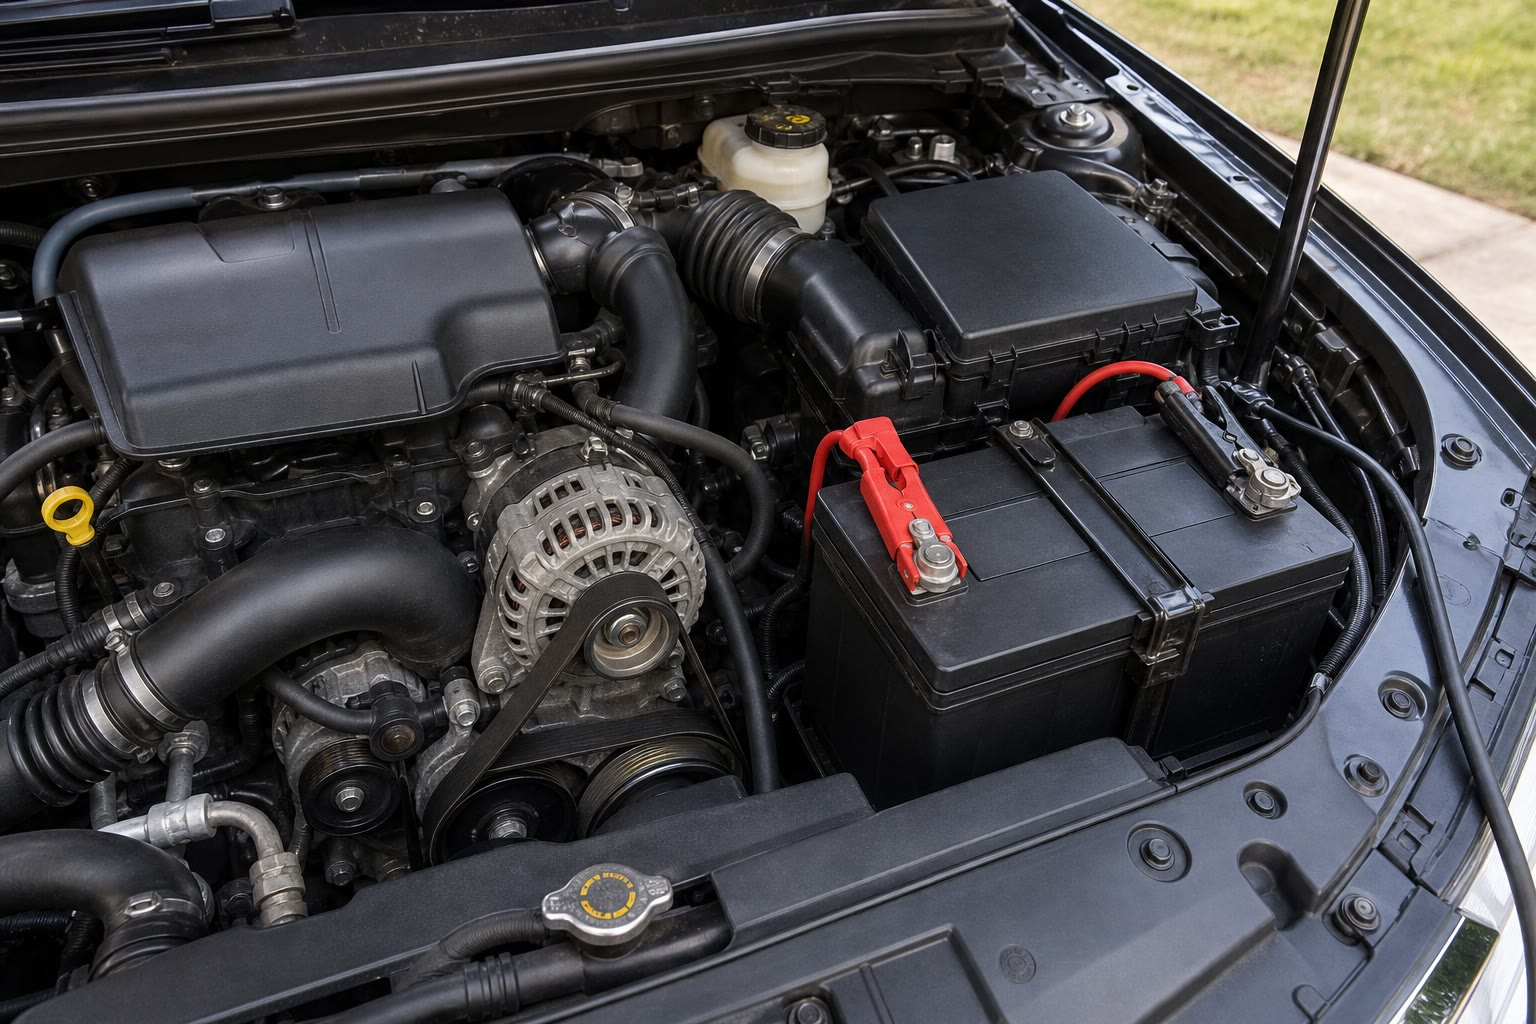
\includegraphics[width=0.58\linewidth]{images/book3/ai/b3-06-car-battery-engine-bay.jpg}

{\small 引擎盖下：\qty{12}{V} 电池、粗电缆与交流发电机——即周末问题中的直流网络，起动瞬间的电流可达数百\omterm{def:b1:dc-circuits:current}{安培}。}
\end{omfigure}

\section{问题：汽车电气系统}

\begin{problem}[{周末问题——一节电池、一台起动机、两盏车灯、
一台交流发电机以及数米铜导线：电流如何分配，谁承担损耗，
以及发动机起动时车灯为何变暗}]
\label{pb:b1:dc-circuits:1}
电池为实际电源，\omterm{def:b1:dc-circuits:sources}{电动势} $E = \qty{12.6}{V}$，\omterm{def:b1:dc-circuits:sources}{内
阻} $r = \qty{10}{m\ohm}$。铜的电阻率：$\rho = \qty{1.7e-8}{\ohm.m}$。

\medskip
\noindent\textbf{第一部分——仅有电池。}
\begin{enumerate}
  \item 画出\omterm{def:b1:dc-circuits:sources}{戴维南模型}，并在
        发电机约定下写出 $u(i)$。
  \item 给出开路\omterm{def:b1:dc-circuits:voltage}{电压}与短路电流。
        为什么掉落的扳手绝不能跨接在接线柱上？
  \item 写出同一电池的\omterm{def:b1:dc-circuits:sources}{诺顿模型}。
  \item 电池向电阻 $R$ 供电：用表达式给出电流、
        端\omterm{def:b1:dc-circuits:voltage}{电压}、输送给电阻的功率 $P_R$，以及在
        $r$ 中损耗的功率。
  \item 证明 $P_R$ 在 $R = r$ 时最大，并求出
        该最大值。此时效率为多少？
  \item 技师测得：电流为 \qty{12}{A} 时 $u = \qty{12.48}{V}$，
        电流为 \qty{120}{A} 时 $u = \qty{11.40}{V}$。验证这两个点都位于
        该模型上，并说明如何由一系列这样的数据点，
        通过直线拟合得到 $E$ 和 $r$。
  \item 电池存储量为 \qty{60}{A.h}。若只让
        两盏 \qty{55}{W} 车灯工作（取 \qty{12}{V}），能维持多长时间？
        这相当于多少焦耳的能量？
\end{enumerate}

\medskip
\noindent\textbf{第二部分——开灯起动。}
起动机为一个电阻 $R_s = \qty{80}{m\ohm}$；每盏车灯
额定功率为 \qty{55}{W}，额定\omterm{def:b1:dc-circuits:voltage}{电压}为 \qty{12.0}{V}，并视为电阻处理。
\begin{enumerate}[resume]
  \item 求一盏车灯的电阻，以及两盏车灯
        并联后的电阻。
  \item 仅起动机工作：求电流、端\omterm{def:b1:dc-circuits:voltage}{电压}、起动机的功率，
        以及电池中损耗的功率。
  \item 起动机与两盏车灯同时工作：求等效负载
        电阻、总电流和端\omterm{def:b1:dc-circuits:voltage}{电压}。
  \item 利用分流公式求起动机电流以及
        车灯电流。
  \item 求每盏车灯现在获得的功率，并与
        其额定值比较：车灯变暗了多少比例？
  \item 用两句话，利用回路定律解释车灯
        变暗的原因正是起动机汲取了较大的电流。
  \item 加粗电池电缆能否使车灯变亮？请先
        定性说明理由（第四部分将作定量分析）。
\end{enumerate}

\medskip
\noindent\textbf{第三部分——发动机运转：交流发电机。}
交流发电机是第二个实际电源，$E_a = \qty{14.2}{V}$，
$r_a = \qty{50}{m\ohm}$，与蓄电池并联；起动机
关闭，两盏前照灯均开启。
\begin{enumerate}[resume]
  \item 画出电路：两个实际电源与前照灯负载
        并联在同样的两个节点之间。
  \item 应用米尔曼定理求公共端\omterm{def:b1:dc-circuits:voltage}{电压}。
  \item 由此求出交流发电机电流、蓄电池电流（注意符号！）以及
        前照灯电流；检验节点定律。
  \item 蓄电池是在充电还是放电？它接收的功率是多少，
        交流发电机提供的功率又是多少？
  \item 用叠加定理重新求出端\omterm{def:b1:dc-circuits:voltage}{电压}（每个电源
        单独作用，另一个以其\omterm{def:b1:dc-circuits:sources}{内阻}代替），并加以
        检验。
\end{enumerate}

\medskip
\noindent\textbf{第四部分——传感器与导线。}
\begin{enumerate}[resume]
  \item 冷却液传感器是一个热敏电阻，其阻值从
        \qty{2.0}{k\ohm}（\qty{20}{\degreeCelsius} 时）降到 \qty{300}{\ohm}（
        \qty{90}{\degreeCelsius} 时）；它是由 \qty{5.0}{V} 供电的\omterm{prop:b1:dc-circuits:dividers}{分压器}中
        下方的电阻，上方的电阻为 $R_0$。写出
        输出\omterm{def:b1:dc-circuits:voltage}{电压}的表达式，并在
        $R_0 = \qty{775}{\ohm}$ 时计算两个温度下的输出\omterm{def:b1:dc-circuits:voltage}{电压}。
  \item 证明：当 $R_0$ 取传感器两个阻值的几何平均值时，
        两个温度之间的输出\omterm{def:b1:dc-circuits:voltage}{电压}变化幅度
        最大，并检验上面的取值。
  \item 将同一传感器接入\omterm{prop:b1:dc-circuits:wheatstone}{惠斯通电桥}，另外三个电阻均为
        \qty{775}{\ohm}：写出电桥的输出\omterm{def:b1:dc-circuits:voltage}{电压}，并说明
        电桥在什么温度下平衡。
  \item 起动机电缆单程长 \qty{1.5}{m}。计算横截面积为 \qty{16}{mm^2} 的
        一根导体的电阻、
        \qty{140}{A} 时的总\omterm{def:b1:dc-circuits:voltage}{电压}降，以及电缆中
        耗散的功率。
  \item 改用 \qty{4}{mm^2} 的电缆重算：起动机电缆为什么这么粗？
  \item 总结：给出起动期间的端\omterm{def:b1:dc-circuits:voltage}{电压}、
        到达起动机的功率所占比例，以及
        解释灯光变暗的那一条定律。
\end{enumerate}
\end{problem}
